\documentclass[a4paper,10pt]{article}
\usepackage[a4paper, total={5.5in, 8.5in}]{geometry}	% define width and height of text part of a page
\usepackage[utf8x]{inputenc}
\usepackage{array}
\usepackage[pdftex]{graphicx}
\usepackage{listings}
\usepackage{enumitem}
\usepackage{color, colortbl}
\usepackage{longtable}
\usepackage{float}
\usepackage[ddmmyyyy]{datetime}
\usepackage[compact]{titlesec}		% The 'compact' argument reduces spacing before and after headings

% Start ---- Fix for bug in issue 2.10.1 of titlesec package
\usepackage{etoolbox}

\makeatletter
\patchcmd{\ttlh@hang}{\parindent\z@}{\parindent\z@\leavevmode}{}{}
\patchcmd{\ttlh@hang}{\noindent}{}{}{}
\makeatother
% End ---- Fix for bug in issue 2.10.1 of titlesec package

\usepackage{verbatim}
\usepackage{fancyhdr}
\usepackage{datatool}	% Management of external databases
\usepackage{chngcntr}	% Management of figure and table numberings
\usepackage{pdflscape}	% Provides 'landscape mode' for selected pages
\usepackage{hyperref}


%---------------------------------------------
% Management of Figure and Table Numbering
%---------------------------------------------
\counterwithin{figure}{section}
\counterwithin{table}{section}

%---------------------------------------------
% Management of Captions (options interact with each other in unpredictable ways)
%---------------------------------------------
\usepackage[labelfont=bf]{caption}	% The caption label for tables and figures is bolded
\setlength{\abovecaptionskip}{2pt}	% Bring caption close to figure or table
\setlength{\belowcaptionskip}{-8pt}	% Bring caption close to text after it
\renewcommand{\figurename}{Fig.}	% The caption label for figures is: "Fig."
%\captionsetup[table]{singlelinecheck=off,justification=raggedright}	% Justify the table captions to the left
\captionsetup[table]{position=bottom,skip=-1pt}	% controls spacing between caption and table
%\captionsetup[figure]{position=bottom,skip=40pt}	

\pagestyle{fancy}

%------------------------------------------------------------------------------------------
% Directories holding image files:
% - Figures from CORDET FW Project
% - Figures from CHEOPS Project
% - Figures from FW Profile Project
%------------------------------------------------------------------------------------------
\graphicspath{ {../images/} }	

%---------------------------------------------
% Paragraph Layout
%---------------------------------------------
\setlength{\parindent}{0in}			% No indentation on first line of a new paragraph

%---------------------------------------------
% Table Layout
%---------------------------------------------
\setlength{\extrarowheight}{1.5pt}	% Add vertical space at a table row
 
 %---------------------------------------------
% Management of changes
%---------------------------------------------
\newcommand{\chgB}[1]{{\color{red}{#1}}{}} 		% Changes in version 2

%------------------------------------------------------------------------------------------
% Management of Headings
%------------------------------------------------------------------------------------------
% Define spacing to the left, before and after a subsection heading
%\titlespacing\subsubsection{8pt}{12pt plus 4pt minus 2pt}{-10pt plus 0pt minus 0pt}
\titlespacing\subsubsection{0pt}{5pt}{0pt}
\titlespacing\subsection{0pt}{5pt}{0pt}

% Introduce a page break before each section
\let\stdsection\section
\renewcommand\section{\newpage\stdsection}

%---------------------------------------------
% Definition of custom properties
%---------------------------------------------
\newcommand{\docIssue}{0.1}						% issue number
\newcommand{\docRefNumber}{PP-DF-COR-0003}		% document reference number

%---------------------------------------------
% Headers and Footers
%---------------------------------------------
\renewcommand{\headrulewidth}{0.4pt}
\renewcommand{\footrulewidth}{0.4pt}

\lhead{\docRefNumber{}}
\chead{}
\rhead{Revision \docIssue{}}
\lfoot{\textcopyright2014 P\&P Software GmbH. All Rights Reserved.}
\cfoot{\vspace{5mm}
%{\color{red}\verbatiminput{../commercial/LicensedTo.txt}}
}
\rfoot{\thepage}
\renewcommand{\headrulewidth}{0.4pt}
\renewcommand{\footrulewidth}{0.4pt}

%---------------------------------------------
% Management of lists
%---------------------------------------------
\setlist{nolistsep}								% No extra vertical space around a list		
\newenvironment{fw_itemize}						% Control spacing between items in a list
{\begin{itemize}
  \setlength{\itemsep}{1mm}
  \setlength{\parskip}{0pt}
  \setlength{\parsep}{0pt}}
{\end{itemize}}

\newenvironment{fw_enumerate}					% Control spacing between items in an enumeration
{\begin{enumerate}
  \setlength{\itemsep}{1mm}
  \setlength{\parskip}{0pt}
  \setlength{\parsep}{0pt}}
{\end{enumerate}}

\newenvironment{fw_description}					% Control spacing between items in a description
{\begin{description}
  \setlength{\itemsep}{1mm}
  \setlength{\parskip}{5pt}			% Line spacing between paragraphs in an item
  \setlength{\parsep}{0pt}}
{\end{description}}

%---------------------------------------------
% Definition of colours
%---------------------------------------------
\definecolor{dkgreen}{rgb}{0,0.6,0}
\definecolor{gray}{rgb}{0.5,0.5,0.5}
\definecolor{light-gray}{gray}{0.85}
\definecolor{mauve}{rgb}{0.58,0,0.82}
\definecolor{lightblue}{RGB}{128,179,255}
\definecolor{lbcolor}{rgb}{0.9,0.9,0.9}

%------------------------------------------------------
% Management of text which is conditionally included
%------------------------------------------------------
\newcommand{\umOnly}[1]{#1}
\renewcommand{\umOnly}[1]{} %Comment out this whole line to suppress exclusion.

\newcommand{\iaswOnly}[1]{#1}
%\renewcommand{\iaswOnly}[1]{} %Comment out this whole line to suppress exclusion.

%---------------------------------------------
% Define Environment for Requirement Tables 
% Par #1: The string identifying the requirement category
% Par #2: The table caption
%---------------------------------------------
\newenvironment{cr_req}[2]
{
\begin{longtable}{|l|p{11.8cm}|}
\caption{#2}\label{tab:Req-#1} \\
\hline
\rowcolor{light-gray}
\textbf{Req. ID} & \textbf{Requirement Text}\\
\hline\hline
\endfirsthead
\rowcolor{light-gray}
\textbf{Req. ID} & \textbf{Requirement Text}\\
\hline\hline
\endhead
\DTLforeach*[\DTLiseq{\cat}{#1}]{dbReq}{\cat=Category,\type=Type,\id=Id,\reqText=Text}
{\DTLiffirstrow{}{\\\hline}P-\cat-\id/\type & \textit{\reqText}}\\\hline
}
{\end{longtable}}

%---------------------------------------------
% Define Environment for Adaptation Point Tables 
% Par #1: The string identifying the category to which the AP applies
% Par #2: The table caption
%---------------------------------------------
\newenvironment{cr_ap}[2]
{
\begin{longtable}{|l|p{4.7cm}|p{6.9cm}|}
\caption{#2}\label{tab:AP-#1} \\
\hline
\rowcolor{light-gray}
\textbf{AP ID} & \textbf{Adaptation Point} & \textbf{Default Value}\\
\hline\hline
\endfirsthead
\rowcolor{light-gray}
\textbf{AP ID} & \textbf{Adaptation Point} & \textbf{Default Value}\\
\hline\hline
\endhead
\DTLforeach*[\DTLiseq{\cat}{#1}]{dbAP}{\cat=Category,\origin=Origin,\id=Id,\ap=AP,\defValue=DefValue}
{\DTLiffirstrow{}{\\\hline}P-\cat-\id & \ap (\origin) & \defValue}\\\hline
}
{\end{longtable}}

%---------------------------------------------
% Define Environment for Observable Tables 
% Par #1: The string identifying the category to which the observable belongs
% Par #2: The table caption
%---------------------------------------------
\newenvironment{cr_obs}[2]
{
\begin{longtable}{|l|p{9.5cm}|}
\caption{#2}\label{tab:Obs-#1} \\
\hline
\rowcolor{light-gray}
\textbf{Name} & \textbf{Description}\\
\hline\hline
\endfirsthead
\rowcolor{light-gray}
\textbf{Name} & \textbf{Description}\\
\hline\hline
\endhead
\DTLforeach*[\DTLiseq{\cat}{#1}]{dbObs}{\cat=Category,\name=Name,\desc=Desc}
{\DTLiffirstrow{}{\\\hline}\texttt{\name} & \desc}\\\hline
}
{\end{longtable}}

%---------------------------------------------
% Define Environment for Parameter Tables 
% Par #1: The string identifying the category to which the parameter belongs
% Par #2: The table caption
%---------------------------------------------
\newenvironment{cr_par}[2]
{
\begin{longtable}{|l|p{9.5cm}|}
\caption{#2}\label{tab:Par-#1} \\
\hline
\rowcolor{light-gray}
\textbf{Name} & \textbf{Description}\\
\hline\hline
\endfirsthead
\rowcolor{light-gray}
\textbf{Name} & \textbf{Description}\\
\hline\hline
\endhead
\DTLforeach*[\DTLiseq{\cat}{#1}]{dbPar}{\cat=Category,\name=Name,\desc=Desc}
{\DTLiffirstrow{}{\\\hline}\texttt{\name} & \desc}\\\hline
}
{\end{longtable}}


%---------------------------------------------
% Import tables with requirements and adaptation points
%---------------------------------------------
\DTLloaddb{dbPus}{PusCompliance.csv}
\DTLloaddb{dbAP}{PusExtensionAP.csv}
\DTLloaddb{dbReq}{PusExtensionReq.csv}
\DTLloaddb{dbObs}{PusExtensionObs.csv}
\DTLloaddb{dbPar}{PusExtensionPar.csv}
\DTLloaddb{dbErr}{PusExtensionErr.csv}
\DTLloaddb{dbReqVerFailCodes}{PusExtensionReqVerFailCodes.csv}

%---------------------------------------------
% Pdf Properties
%---------------------------------------------
\hypersetup
{
    pdfauthor={Alessandro Pasetti},
    pdfsubject={This document specifies the PUS Extension of the CORDET Framework},
    pdftitle={PUS Extension of the CORDET Framework},
    pdfkeywords={PUS, CORDET}
}

%---------------------------------------------
% Title Page
%---------------------------------------------
\title{\textsc{The CORDET Framework} \\ \textsc{- PUS Extension -}}
\author{Alessandro Pasetti }
\date{Created on: \today{}, at: \currenttime{}}

\begin{document}
\maketitle

\begin{center}
Revision \docIssue{}\\
\docRefNumber{}
\end{center}

\vspace{1cm}

\begin{center}
P\&P Software GmbH \\
High Tech Center 1 \\
8274 T\"{a}gerwilen (CH)\\
\vspace{2mm}
Web site: \url{www.pnp-software.com}\\
E-mail: \href{mailto:pnp-software@pnp-software.com}{\nolinkurl{pnp-software@pnp-software.com}} 
\end{center}

\vspace{0.5cm}

\begin{table}[ht]
\begin{center}
\begin{tabular}{p{11.7cm}}
\\
\hline
\end{tabular}
\end{center}
\end{table}
\begin{abstract}
This document specifies the PUS Extension of the CORDET Framework. The CORDET Framework is a software framework for service-oriented embedded applications. The service concept of the CORDET Framework is the same as the service concept of the Packet Utilization Standard or PUS. The PUS is an application-level interface standard for space-based distributed systems.

The PUS pre-defines a number of services. This document extends the CORDET Framework to support a subset of those services. The document specifies the components which implements them. The components are specified by providing their behavioural model. The behavioural models are defined using the FW Profile.

\end{abstract}
\begin{table}[ht]
\begin{center}
\begin{tabular}{p{11.7cm}}
\\
\hline
\end{tabular}
\end{center}
\end{table}


\newpage
\vspace*{\fill}
\begin{center}
No part of this publication may be reproduced, transmitted, transcribed, stored in any retrieval system, or translated into any language by any means without express prior written permission of P\&P Software GmbH.
\end{center}

\begin{center}
Copyright \textcopyright 2014 P\&P Software GmbH. All Rights Reserved. 
\end{center}
\vspace*{\fill}

%---------------------------------------------
% Table of Contents
%---------------------------------------------
\newpage
\tableofcontents

\newpage
\listoffigures
\listoftables

\newpage

%---------------------------------------------
% Adjust distance between paragraphs (this cannot be done earlier or it also affects the TOC)
%---------------------------------------------
\setlength{\parskip}{3mm}						% Set distance between paragraphs

%==========================================================================================
\section{Change History}

This section lists the changes made in the current and previous revisions. Changes are classified according to their type. The change type is identified in the second column in the table according to the following convention:

\begin{fw_itemize}
\item "\textbf{E}": Editorial or stylistic change
\item "\textbf{L}": Clarification of existing text
\item "\textbf{D}": A requirement has in whole or in part been deleted
\item "\textbf{C}": A requirement has been modified
\item "\textbf{N}": A new requirement has been introduced
\item "\textbf{T}": A TBD or TBC has been resolved
\end{fw_itemize}

Text which is new or has been modified in the current revision is in red font. If a figure has been modified, then its caption is in red font. Section header numbers do not change from one revision to the next (but new sections may, of course, be introduced). However, figure and table numbers may change and these changes are not tracked. Changes in the appendices are not tracked as they are consequences of changes in the main body of the document.

\begin{longtable}{|c|c|p{10cm}|}
\caption{Detailed List of Changes in Issue 0.1} \\
\hline
\rowcolor{light-gray}
\textbf{Sec} & \textbf{Type} & \textbf{Description of Change} \\
\hline\hline
\endfirsthead
\rowcolor{light-gray}
\textbf{Sec} & \textbf{Type} & \textbf{Description of Change} \\
\hline\hline
\endhead
n.a. & L & This is the first release of this document \\
\hline
\end{longtable}






\newpage

%==========================================================================================
\section{Applicable and Reference Documents}

The documents in table \ref{tab:appDoc} form an integral part of the present document. The documents in table \ref{tab:refDoc} are referenced in the present document and are for information only.

\begin{longtable}{|c|p{11cm}|}
\caption{Applicable Documents} \label{tab:appDoc}\\
\hline
\rowcolor{light-gray}
\textbf{ID} & \textbf{Title, Reference Number, Revision Number} \\
\hline\hline
\endfirsthead
\rowcolor{light-gray}
\textbf{ID} & \textbf{Title, Reference Number, Revision Number} \\
\hline\hline
\endhead
[CR-SP] & The CORDET Framework - Specification, PP-DF-COR-00002, Revision 1.6, P\&P Software GmbH, Switzerland, 2012, Available from: \url{www.pnp-software.com/cordetfw} \\
\hline
[FW-SP] & The Framework Profile, PP-DF-COR-00001, Revision 1.3, P\&P Software GmbH, Switzerland, 2012, Available from: \url{www.pnp-software.com/fwprofile} \\
\hline
[PS-SP] & Ground Systems and Operations – Telemetry and Telecommand Packet Utilization Standard, ECSS-E-70-41C, April 2016, European Cooperation for Space Standardization (ECSS) \\
\hline
\end{longtable}

\begin{longtable}{|c|p{11cm}|}
\caption{Reference Documents} \label{tab:refDoc}\\
\hline
\rowcolor{light-gray}
\textbf{ID} & \textbf{Title, Reference Number, Revision Number} \\
\hline\hline
\endfirsthead
\rowcolor{light-gray}
\textbf{ID} & \textbf{Title, Reference Number, Revision Number} \\
\hline\hline
\endhead
[PS-WEB] & The CORDET Framework Project Web Site Profile, \url{www.pnp-software.com/cordetfw} \\
\hline
\end{longtable}


\newpage


%==========================================================================================
\section{Introduction}
The CORDET Framework is a software framework for service-oriented embedded applications. It is specified in AD-1 as a set of components to manage the services which an application provides to other applications and uses from other applications. A C-language implementation of this specification is available from RD-1.

The CORDET Framework only covers the management of generic services but does not specify any concrete services. The service concept of the CORDET Framework is the same as the service concept of the \textit{Packet Utilization Standard} (PUS). The PUS is an application-level interface standard for space-based distributed systems. It is defined in AD-3.

The PUS pre-defines a number of services. This document extends the CORDET Framework to support a subset of those services. The document specifies the components which implements them. The components are specified by providing their behavioural model. The behavioural models are defined using the FW Profile. The FW Profile is a UML profile for reusable software components. It is defined in AD-2.

The set of components specified in this document are called the \textit{PUS Extension of the CORDET Framework}. When there is no danger of ambiguity, the shorter names "framework extension" or "PUS extension" are also used as synonyms of PUS Extension of the CORDET Framework.

In terms of the classical software lifecycle, the specification presented in this document is at the level of software requirements in the sense that it defines a complete and unambiguous logical model of the components implementing the PUS extension of the CORDET Framework.

\textbf{This document assumes the reader to be familiar with the specification of the CORDET Framework in AD-1}. 

\subsection{Scope of CORDET Framework}\label{sec:ScopeCrFw}
A \textit{CORDET service} is a set of logically and functionally related capabilities that an application offers to other applications (see section 2.2 of AD-1). The CORDET Service concept sees an application as a \textit{provider of services} to other applications and as a \textit{user of services} from other applications (see figure \ref{fig:ServConcept}).

\begin{figure}[ht]
 \centering
 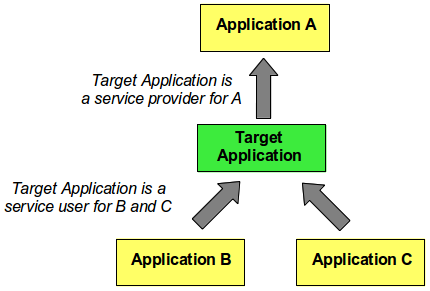
\includegraphics[scale=0.4,keepaspectratio=true]{ServConcept.png}
 \caption{Applications as Providers and Users of Services}
 \label{fig:ServConcept}
\end{figure}

The user of a service controls the service by sending \textit{commands} to the service provider. A command is a data exchange between a service user and a service provider to control the execution of a particular activity within the service provider. 

The provider of a service sends \textit{reports} to the user of the service. A report is a data exchange between a service provider (the report initiator) and a service user to provide information relating to the execution of a service activity.

Thus, a service consists of a set of commands which the user of the service sends to the provider of the service and of a set of reports which the service provider sends back to its user. A command defines actions to be executed by the service provider. 
A report encapsulates information about the internal state of the service provider.

Against this background, the CORDET Framework of AD-1 fulfils two objectives:

\begin{fw_itemize}
\item{} It provides a formal definition of the abstract command concept and of the abstract report concept by building behavioural models of commands and reports which:
	\begin{fw_itemize}
	\item capture the aspects of the behaviour of commands and reports which is common to all commands and reports independently of the definition and implementation of a concrete command or report, and
	\item identify the adaptation points where service- and implementation-specific behaviour can be added.
	\end{fw_itemize}
\item{} It specifies the the component (the \textit{CORDET Components}) which implement the abstract command and report concepts.
\end{fw_itemize}

The CORDET Components cover, on the service user side, the sending of commands and the reception and distribution of reports and, on the service provider side, the processing of incoming commands and the generation of reports but do not cover the implementation of any concrete services. 

%--------------------------------------------------------------------------------
\subsection{Scope of PUS Extension of CORDET Framework}\label{sec:ScopePusExt}
Developers of a CORDET application are expected to deploy the CORDET components and complement them with application-specific components which implement the services of interest to them. The PUS extension of the CORDET Framework is intended to facilitate the task of application developers by offering them a set of pre-defined components which implement a set of \textit{Standard Services}. A standard service in this context is a service which implements commonly used functions within a certain domain. 

The standard services of the PUS Extension are taken from the Packet Utilization Standard (PUS) of AD-3. The target domain of the PUS Extension is therefore that of space-borne service-provider applications but it is worth stressing that the set of services selected from the PUS are those which are least dependent on the space context and it is therefore expected that the services implemented by the PUS Extension may be of interest to other application domains.

The standard services are defined by defining their commands and reports and the commands and reports are defined as specializations of the abstract command and report concepts of the CORDET Framework. Thus, a standard service is defined by “closing” the adaptation points identified in the abstract command and report concepts.

The CORDET Framework is ultimately intended to foster reuse (at both specification and implementation level) in the field of service-oriented embedded applications. The reuse model it promotes is illustrated in figure \ref{fig:HierarchicalDefServ}. 
At the top layer, there is the abstract definition of commands and reports of the CORDET Framework of AD-1. This definition is entirely generic and applicable to all services in all application. At the intermediate level, standard services are defined which capture concrete behaviour which is common to a large number of applications. The present document specifies one such set of standard services. Finally, at the bottom level, end-applications define their own services which are entirely specific to their needs. The application-level services may be either taken over from the standard services or they may be created as instantiations of the generic service concept (if they are entirely application-specific).

Note that the PUS Extension of the CORDET Framework specifies several services. These services are specified to be independent of each other so that the user may choose only a subset of these services. Similarly, each service is specified in terms of the commands and reports which implement it. Dependencies among the commands and reports of a service are minimized so that user may be free to import into their application just a subset of the commands and reports of a given service.

\begin{figure}[ht]
 \centering
 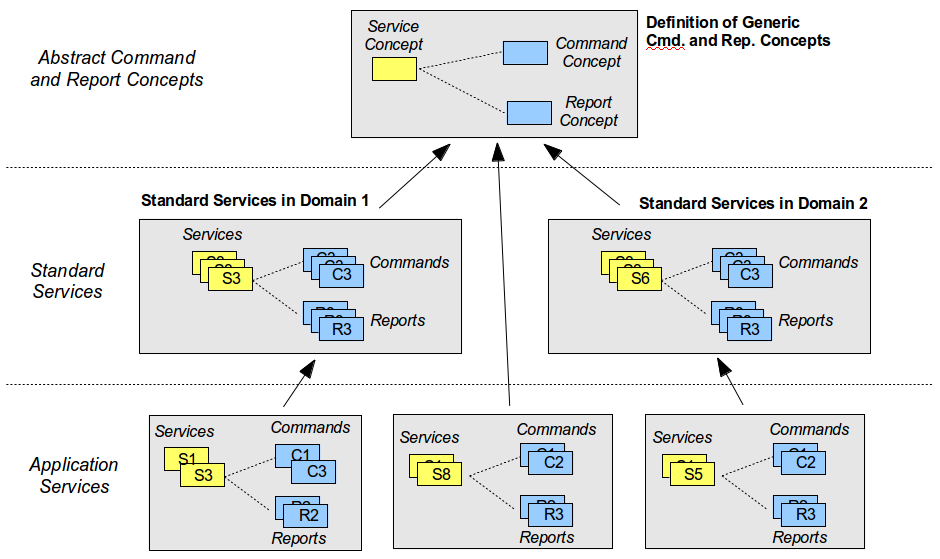
\includegraphics[scale=0.3,keepaspectratio=true]{HierarchicalDefServ.png}
 \caption{Hierarchical Definition of Services}
 \label{fig:HierarchicalDefServ}
\end{figure}


%---------------------------------------------------------------------------------
\subsubsection{Overview of Supported Services}
Table \ref{tab:supportedServ} lists the services supported by the PUS Extension of the CORDET Framework. The first column gives the service type identifier. The last column points to the section in this document where the support for the service is specified.

\begin{longtable}{|c|>{\raggedright\arraybackslash}p{6cm}|c|}
\caption{Services Supported by PUS Extension}\label{tab:supportedServ} \\
\hline
\rowcolor{light-gray}
\textbf{N} &\textbf{Service} & \textbf{Section} \\
\hline\hline
\endfirsthead
\rowcolor{light-gray}
\textbf{N} &\textbf{Service} & \textbf{Section} \\
\hline\hline
\endhead
1 & Request Verification Service & \ref{sec:serv1} \\
\hline
3 & Housekeeping Service & \ref{sec:serv3} \\
\hline
TBD & TBD & TBD \\
\hline
\end{longtable} 


%------------------------------------------------------------------------------------
\subsection{Specification Format} 
This document specifies the PUS Extension of the CORDET Framework. The framework is specified by defining its requirements. The requirements of the framework are of four types:

\begin{fw_itemize}
\item{} \textit{Standard Requirements} which define a desired feature of the framework extension. They are analogous in scope and format to the user requirements of a conventional (non-framework) application.
\item{} \textit{Adaptation Requirement} which define the points where a component offered by the framework extension can be extended by the application developers. 
In some cases, the definition of an adaptation point is accompanied by the definition of the default options offered by the framework extension for that adaptation point.  
\item{} \textit{Usage Constraint Requirements} which define the constraints on how the components offered by the framework extension may be used by application developers.
\item{} \textit{Property Requirements} which define behavioural properties which are guaranteed to hold on all applications which: (a) are instantiated from the CORDET Framework and its extension by closing their adaptation points, and (b) comply with the framework's usage constraints.
\end{fw_itemize}

To each framework requirement an \textit{identifier} is attached.
The requirement identifier takes the following form: x-y/t where 'x' is an acronym identifying the function to which the requirement applies; 'y' is a unique identifier within that function; and 't' identifies the requirement type. 
The type is designated by one single letter as follows: 'S' for the Standard Requirements, 'A' for the Adaptation Requirements, 'C' for the Usage Constraint Requirements and 'P' for the Property Requirements.

The specification of the framework extension includes a \textit{behavioural model} of the framework which describes its behaviour and identifies the adaptation points where application developers can extend this behaviour to match their requirements.  

The behavioural model of the framework extension is defined using the FW Profile of AD-2. 
It therefore consists of a set of \textit{state machines} (represented as state charts) and \textit{procedures} (represented as  activity diagrams). 
Familiarity with the FW Profile is essential for a full understanding of the framework requirements.

Wherever possible, the framework extension requirements simply make the state machines and procedures applicable. In other words, the state charts representing state machines and the activity diagrams representing procedures are treated as normative and no attempt is made to translate them into a comprehensive set of equivalent requirements.

In accordance with the FW Profile, the activity diagrams and state diagrams identify the framework adaptation points using the <<AP>> stereotype (but note that not all adaptation points are identified explicitly in activity or state diagrams). 
For convenience, all adaptation points with their default options are listed in dedicated tables. 
In most cases, the adaptation requirements simply make the items in such tables applicable. By default, the implementation mechanism for the adaptation points is left open and is not covered by this specification. 

Some of the components specified by the framework extension are defined as extensions of CORDET components. In such cases, the extended component is derived from the base component by either \textit{overriding} or \textit{closing} some of its adaptation points. 
A derived component overrides an adaptation point of its base component when it changes the default behaviour associated to that adaptation point (but applications can still change that behaviour). 
A derived component closes an adaptation point of its base component when it defines in a final way the behaviour associated to that adaptation point (i.e. applications can no longer change that behaviour).

%----------------------------------------------------------------------------------
\subsection{Compliance to PUS Requirements}\label{sec:ComplianceToPus}
The PUS Extension of the CORDET Framework implements a subset of the standard PUS services of AD-3. In order to provide visibility over the level of compliance to the PUS requirements of AD-3, appendix \ref{sec:PusReqSOC} presents a statement of compliance to these requirements. This demonstrates that, for the selected services, the PUS Extension is fully compliance to the PUS requirements.


%=============================================================================================
\section{Report and Command Attributes}\label{sec:repCmdAttr}
The CORDET Framework defines a number of attributes for commands and reports. Table \ref{tab:pcktAttPus} shows how they are mapped to the command and report attributes defined by the PUS. In most cases, the mapping is straightforward but, in the case of the discriminant and of the APID, clarifications are in order which are provided in the next two sub-sections. 

The PUS Extension of the CORDET Framework extends the range of command and report attributes to include all command and report attributes defined by the PUS. Thus, the components defined by the framework extension to implement PUS commands and reports provide operations to access all the attributes defined at PUS level. 

Within the framework, commands and reports are handled as instances of components of type InReport (for incoming reports), InCommand (for incoming command), or OutComponent (for out-going commands and reports). Commands and reports arrive at and leave the framework throughthe OutStream and InStream components, which constitute the external interfaces of the framework. At these interfaces, commands and reports are instead encapsulated in packets (sequences of bytes which carry all the data in the report or command). In the framework extension, these packets are required to comply to the command and report layout defined by the PUS and the framework extension is required to provide operation to encode and decode the packets, i.e. to set and read the values of any PUS-defined parameter in a packet. 

\begin{longtable}{|c|>{\raggedright\arraybackslash}p{11cm}|}
\caption{CORDET-PUS Attribute Mapping}\label{tab:pcktAttPus} \\
\hline
\rowcolor{light-gray}
\textbf{Attribute} & \textbf{Mapping to PUS Attribute} \\
\hline\hline
\endfirsthead
\rowcolor{light-gray}
\textbf{Attribute} & \textbf{Mapping to PUS Attribute} \\
\hline\hline
\endhead
\texttt{Src} & Commands: source field of data field header; Reports: PID \\
\hline
\texttt{Dest} & Commands: PID; Reports: destination field of data field header \\
\hline
\texttt{SeqCnt} & Sequence Count field in packet header \\
\hline
\texttt{CmdRepType} & Packet Type bit in packet header \\
\hline
\texttt{Length} & Related to Packet Length Field (which is the length of the packet data field minus 1) \\
\hline
\texttt{TimeStamp} & Time Field in data field header of telemetry packets; not present in telecommand packets \\
\hline
\texttt{Discriminant} & Service-specific mapping to parameter which determines command or report layout, see section \ref{sec:mapDisc} \\
\hline
\texttt{ServType} & Service Type field in data field header \\
\hline
\texttt{ServSubType} & Service Sub-Type field in data field header \\
\hline
\texttt{Group} & Related to CAT part of the APID, see section \ref{sec:mapGroup} \\
\hline
\texttt{CmdRepId} & Not present \\
\hline
\texttt{AcceptAck} & Bit 3 of acknowledge field in data field header \\
\hline
\texttt{StartAck} & Bit 2 of acknowledge field in data field header \\
\hline
\texttt{ProgressAck} & Bit 1 of acknowledge field in data field header \\
\hline
\texttt{TermAck} & Bit 0 of acknowledge field in data field header \\
\hline
\texttt{ParStart} & The parameter area starts where the Application Data starts, namely at the 11-th byte of a command packet and at the 17-th byte of a report packet \\
\hline
\texttt{ParLength} & The parameter length is the total packet length (in bytes) minus 10 for command packets and the total packet length (in bytes) minus 16 for report packets \\
\hline
\end{longtable}  


%----------------------------------------------------------------------------------
\subsection{Mapping of Discriminant Attribute}\label{sec:mapDisc}
The CORDET discriminant is an optional attribute of a command or report. It is defined when the layout or the behaviour of a command or report are not exclusively determined by the command or report type and sub-type; in such cases, the discriminant becomes the determinant of the command or report layout and behaviour. The PUS does not have the concept of discriminant but some of its services use a particular field for the same purpose. For instance, the Event Identifier (EID) of service 5 reports determines the layout of a service 5 report and hence serves the same purpose as the CORDET discriminant. Similarly, some commands or reports carry variable-length blocks of data; in such cases, the parameter which defines the length of the data block acts as a discriminant. Bearing in mind these considerations, the discriminant is mapped to the following PUS parameters:

\begin{fw_itemize}
\item The SID for (3,25) reports
\item The EID for service 5 reports
\item TBD
\end{fw_itemize}

%----------------------------------------------------------------------------------
\subsection{Mapping of Group Attribute}\label{sec:mapGroup}
The CORDET Framework does not have the concept of APID but it uses the concept of group to represent it. More precisely, the CORDET Framework assigns sequence counters to commands and reports and assigns commands and reports going through an InStream or OutStream to 'groups'. The CORDET sequence counters are initialized to 1 and are incremented by 1 within each group (i.e. for each group in an OutStream, a counter is maintained which is incremented by 1 whenever a command or report belonging to that group is issued by the OutStream; and for each group in an InStream, a counter is maintained which is incremented by 1 whenever a command or report belonging to that group is received by the InStream). 

The CORDET Framework requires that, for each destination for out-going commands or reports, an OutStream be defined and that, for each source of incoming commands or reports, an InStream be defined. 

Bearing in mind the above, compliance with the PUS rules for the management of the sequence counters requires that the following rules be adopted for the assignment of the groups: 

\begin{fw_itemize}
\item If an application sends commands or reports to the same destination with different APIDs, then for each such APID, a group must be defined
\item If an application receives commands or reports from the same source  with different APIDs, then for each such APID, a group must be defined
\end{fw_itemize}


%----------------------------------------------------------------------------------
\newpage
\subsection{Requirements}
The table in this section lists the requirements for the command and report attributes.

\begin{cr_req}{CRA}{Requirements for Command and Report Attributes}
\end{cr_req}
 

%=============================================================================================
\section{The Data Pool Component}\label{sec:dp}
The Data Pool Component is a pre-defined component offered by the PUS Extension of the CORDET Framework. It is used by all services supported by the framework extension and it is therefore defined independently of these services.

%-----------------------------------------------------------------------------
\subsection{Data Pool Concepts}\label{sec:dpConcepts}
The Data Pool Component provides read-write access to a set of \textit{Data Items}. A Data Item is characterized by the following attributes: 

\begin{fw_itemize}
\item \textit{Default Value}: the value of the data item when the data pool is reset
\item \textit{Current Value}: the value of the data item at a particular point in time
\item \textit{Identifier}: a positive integer which uniquely identifies the Data Item within the Data Pool
\item \textit{Type}: an enumerated value which determines the range of possible values of the Data Item and its representation in the Data Pool
\end{fw_itemize}

With reference to the last bullet, it is noted that the set of supported types is defined at implementation level. The data items can be of two kinds:

\begin{fw_itemize}
\item \textit{Parameters}: data items whose value is under the control of an entity external to the host application 
\item \textit{Variables}: data items whose value is autonomously updated by the host application as part of its normal operation
\end{fw_itemize}

In practice, the data pool is the means through which a component can access data belonging to other components. Note that this specification is silent about the physical location of the data items in the data pool, which can be either the components which own the data item (in which case the data pool only offers a link to the data items), or the data pool itself, or a mixed solution where some data items reside in the data pool and others in peripheral components. 

This specification is similarly silent about the internal structure of data items and, in particular, it neither restricts them to be of primitive type nor does it mandate an array-like structure for them. Any such restrictions or options must be introduced at implementation level.

%---------------------------------------------------------------------------------
\subsection{Data Pool Behaviour}\label{sec:dpBehaviour}
The Data Pool Component - like all other CORDET Components - is an extension of the Base Component of section 3.2 of AD-1. It does not add any behaviour to the Base Component but it specializes some of its adaptation points as described below.

The Initialization Procedure of the Data Pool Components creates the data structures needed by the component. At one extreme, if an implementation chooses to locate all data items inside the Data Pool Component, then its Initialization Procedure is responsible for creating the data structures which host the data items. At the other extreme, in an implementation where data items remain located in their originating components and where the data pool only acts as a kind of data switch-board, the Initialization Procedure does nothing and always returns "initialization successful".

When the Data Pool is reset, the current values of its data items are initialized with their default values. The Configuration Procedure is therefore responsible for initializing the data item values with their default values. 

This specification does not say where the default values of the data items are stored in relation to their current values. At implementation level, two basic options are possible:

\begin{fw_enumerate}
\item The default values are stored alongside the current values (i.e. in RAM)
\item The default values are stored in some other memory area (e.g. in an EEPROM or in a remote location)
\end{fw_enumerate}

In the first case, the initialization of the data items simply involves a copy across two locations in RAM. in the second case, the initialization may be a potentially lengthy process involving the retrieval of the data item values from an external memory bank or from a remote location. The Data Pool Component covers both options and its Configuration Procedure is therefore defined as follows:

\begin{fw_itemize}
\item The Configuration Action starts the process whereby the default values of the data items are acquired and copied to their current values
\item The Configuration Check returns "success" if the initialization of the data item values can be done in zero logical execution time\footnote{The concept of \textit{logical execution time} is introduced in AD-2 as part of the FW Profile Definition. The logical execution time of a behaviour is the execution time of that behaviour on a processor with infinite speed and in the absence of pre-emption by higher-priority activities or blocking by lower-priority activities. Essentially, a behaviour has zero logical execution time if it includes neither "wait" operations nor synchronization operations with external devices or threads.} or else when the initialization has completed 
\end{fw_itemize}

In the case where the initialization of the data item values is not an operation with zero logical execution time, then the Data Pool Component must be sent at least two \texttt{Reset} commands before it can enter the CONFIGURED state: the first \texttt{Reset} command starts the acquisition of the default values of the data items and the second \texttt{Reset} command verifies that the acquisition has terminated. Obviously, there is nothing to stop an application from using a "polling" approach and sending a sequence of \texttt{Reset} commands until the Data Pool Component has entered its CONFIGURED state. Note that, in line with requirements AST-5 and AST-7 in AD-1, it is the responsibility of the application to send as many \texttt{Reset} commands as needed to the Data Pool Component during the application start-up and application reset process.

No behaviour is associated to the Data Pool Component when it is in state CONFIGURED and hence there is no need to define an Execution Procedure for it.

Finally, the Data Pool Component offers operations to give read-write access to the current values of the data items. The mode of access to these values (through functions which returns pointers to the data items or through functions which return their values) is not specified and is left to the implementation to decide. Also, no limitation is specified on which components can access the data items in the data pool: any component can access any data item in read-write mode. Such limitations, if needed, may be added at implementation level. 

The data item access operation use the Data Item Identifier as the key to identify the data item whose current value is to be read or updated. The behaviour of these operations in case an illegal identifier is used is not specified at framework level but it is noted that the design of the framework components is such that this situation (attempt to access a non-existent data item in the data pool) never arises. 

%---------------------------------------------------------------------------------
\subsection{Service Observability Concept}\label{sec:servObsConcept}
The data pool plays a key role in service 3 (see section \ref{sec:serv3}) but it is also used by other services as the repository through which service observables are accessed. Each service defines a number of \textit{service observables}. These are data items which the service is responsible for keeping up-to-date and which reflect its current state. The service observables are assigned to the data pool which means that they can be accessed using service 3. Note that some of this service status information may also be accessible using service-specific reports (i.e. there may be a degree of redundancy in the observability of the service). 

%---------------------------------------------------------------------------------
\subsection{Service Parameterization Concept}\label{sec:servParConcept}
Each service defines a number of \textit{service parameters}. These are data items which control the behaviour of the service and whose value is set either by the user of the application hosting the service (e.g. the ground) or by other services in the application. Service parameters are assigned to the data pool which means that they can be accessed using service 3. Note that some of the service parameters may also be controlled using service-specific commands (i.e. there may be a degree of redundancy in the commandability of a service).


%---------------------------------------------------------------------------------
\subsection{Adaptation Points}
The table in this section lists the adaptation points for the Data Pool Component.

\begin{cr_ap}{DP}{Adaptation Points for Data Pool Component}
\end{cr_ap}

%---------------------------------------------------------------------------------
\newpage
\subsection{Requirements}
The table in this section lists the requirements for the Data Pool Component.

\begin{cr_req}{DP}{Requirements for Data Pool Component}
\end{cr_req}

%=============================================================================================
\section{Report and Command Factories}\label{sec:repCmdFactories}
Command and report components must be instantiated dynamically as the need arises to generate or process them. For this purpose, the CORDET Framework defines the OutFactory and InFactory components to encapsulate the instantiation process of, respectively, OutComponents and InCommands/InReports. Both kinds of components provide two operations: \texttt{Make} to create an instance of a command or report of a given kind (as given by the triplet [type, sub-type, discriminant]) and \texttt{Release} to release command or report instance.

The CORDET Framework specifies the interface of the factory components but does not actually provide them because it does not provide any concrete command or report components. The framework extension provides concrete commands and reports and is therefore required to also provide implementations of the two factory components.

The process through which the command and report components are created by the factories is not specified. In particular, the allocation policy for the memory for the instantiated components is left open for the implementation to decide.

%---------------------------------------------------------------------------------
\subsection{Observables}
The table in this section lists the variables which are maintained and made accessible through the data pool by the two factory components.

\begin{cr_obs}{FAC}{Data Items for Factory Components}
\end{cr_obs}

%---------------------------------------------------------------------------------
\subsection{Adaptation Points}
The Make and Release operations for the two factory components are adaptation points because the command and report instantiation policies are not defined at framework extension level. These two adaptation points are, however, already defined at CORDET Framework level (see adaptation points FAC-1 and FAC-2 in AD-1) and do not therefore need to be defined again here.

Similarly, the factory components are defined in AD-1 as extension of the Base Component and they they therefore inherit all the adaptation points of the Base Components but no further specialization of these adaptation points in done in the framework extension.

%---------------------------------------------------------------------------------
\subsection{Requirements}
The table in this section lists the requirements for the factory components.

\begin{cr_req}{FAC}{Requirements for Factory Components}
\end{cr_req}


%=============================================================================================
\section{Definition of PUS Reports and Commands}\label{sec:defPusRepCmd}
The PUS Extension of the CORDET Framework supports a subset of the PUS services and, for these services, it specifies the components which implement their reports and commands. Since the framework extension covers the provision of PUS services, it is only concerned with incoming commands and out-going reports. 

In the CORDET Framework, incoming commands are encapsulated by InCommand components and out-going components are encapsulated by OutComponent components. The InCommand and OutComponent components define abstract commands and reports. These two components offer a number of adaptation points where behaviour must be inserted to define concrete commands and reports. A concrete command or a concrete report is specified by closing the adaptation points of, respectively, the InCommand component or of the OutComponent component. 

Thus, for each supported PUS command, the framework extension defines an extension of the InCommand component which closes all the InCommand adaptation points and, for each supported PUS reports, it defined an extension of the OutComponent component which closes all the OutComponent adaptation points.

Table \ref{tab:supportedPus} lists the command and report components provided by the PUS Extension of the CORDET Framework to support the PUS services. The first column in the table gives the name of the CORDET component which implements the command or report and the second column gives its PUS names as it is given in section 8 of [PS-SP].

%--------------------------------------------------------------------------------------
\subsection{Report and Command Adaptation Points}\label{sec:repCmdAP}
Rows 1 to 18 of table \ref{tab:AP-PCR} list the adaptation points of the OutComponent component and describes how they are closed for the PUS reports provided by the framework extension. In some cases, the adaptation point is closed in the same way for all framework reports. In other cases, the close-out is report-specific and is then described in the following sections of this document which define the individual PUS services. Thus, for instance, the close-out of the report-specific adaptation points for the service 1 reports can be found in section \ref{sec:serv1AP}. The following considerations apply to the data in the table:

\begin{fw_itemize}
\item The OutComponent components are created by the OutFactory and it can be assumed that they are created such that they can be successfully initialized and configured. Their initialization and configuration procedures (adaptation points OCM-1 to 4) can therefore be just dummies that do not perform any action. The same applies to the shutdown procedure (adaptation point OCM-5).
\item The adaptation point OCM-6 related to the execution procedure is already closed at CORDET Framework level because OutComponents have no execution procedure.
\item The adaptation points OCM-7 and 8 related to the setting of the report type and sub-type are closed in accordance with the discussion in section \ref{sec:repCmdAttr} by setting the CORDET types and sub-types equal to the PUS type and sub-type.
\item The adaptation points OCM-9 and OCM-10 to 12 related to the setting of the report discriminant, destination and parameters are closed for each individual report type in the following sections of this document.
\item The adaptation point OCM-10 related to the acknowledge level is only relevant to out-going commands and is therefore not applicable to the PUS reports.
\item The adaptation points OCM-13 to 16 related to the report checks and actions are closed for each specific report type in the following sections of this document.
\item The adaptation point OCM-17 related to the serialize operation is closed to create a packet layout which complies with the layout defined by the PUS in [PS-SP].
\item The adaptation point OCM-18 covers the response to a report having an invalid destination. By design, this situation should never arise and the adaptation point is closed with the generation of an error report.
\end{fw_itemize}

In a similar fashion, rows 19 to 39 of table \ref{tab:AP-PCR} list the adaptation points of the InCommand component and describes how they are closed for the PUS commands provided by the framework extension. In some cases, the adaptation point is closed in the same way for all framework commands. In other cases, the close-out is command-specific and is then described in the following sections of this document which define the individual PUS services. Thus, for instance, the close-out of the command-specific adaptation points for the service 17 commands can be found in section \ref{sec:serv17AP}. The following considerations apply to the data in the table:

\begin{fw_itemize}
\item The InCommand components are created by the InFactory but are then initialized and configured by the InLoader. Their initialization and configuration procedures (adaptation points ICM-1 to 4) are therefore implementation-specific. The same applies to the shutdown procedure (adaptation point ICM-5).
\item The adaptation point related to the execution procedure (ICM-6) is already closed at CORDET Framework level because InCommand do not have any execution procedure.
\item The adaptation points ICM-7 to 11 related to the command checks and actions are closed for each specific command type in the following sections of this document.
\item The adaptation point ICM-10 related to the acknowledge level is only relevant to out-going commands and is therefore not applicable to the PUS reports.
\item The adaptation points ICM-12 to 17 related to the generation of success and failure reports for the command are closed as part of the service 1 definition in section \ref{sec:serv1AP}.
\item The adaptation points ICM-18 and 19 related to the setting of the command type and sub-type are closed in accordance with the discussion in section \ref{sec:repCmdAttr} by setting the CORDET types and sub-types equal to the PUS type and sub-type.
\item The adaptation points ICM-20 and 21 related to the command discriminant and parameters are closed for each individual command type in the following sections of this document.
\end{fw_itemize}

\begin{cr_ap}{PCR}{Adaptation Points for PUS Reports and Commands}
\end{cr_ap}

%--------------------------------------------------------------------------------------
\subsection{Requirements}\label{sec:repCmdReq}
The requirements in table \ref{tab:Req-PCR} make the adaptation points defined in the previous two sections applicable to all command and report components provided by the framework extension.

\begin{cr_req}{PCR}{Requirements for Framework Extension Commands and Reports}
\end{cr_req}


\begin{longtable}{|l|>{\raggedright\arraybackslash}p{9cm}||c|}
\caption{Supported PUS Commands and Reports}\label{tab:supportedPus} \\
\hline
\rowcolor{light-gray}
\textbf{CORDET Name} & \textbf{PUS Name} & \textbf{Type} \\
\hline\hline
\endfirsthead
\rowcolor{light-gray}
\textbf{CORDET Name} & \textbf{PUS Name} & \textbf{Type} \\
\hline\hline
\endhead
VerSuccessAccRep & Successful Acceptance Verification Report & (1,1) \\
\hline
VerFailedAccRep & Failed Acceptance Verification Report & (1,2) \\
\hline
VerSuccessStartRep & Successful Start of Execution Verification Report & (1,3) \\
\hline
VerFailedStartRep & Failed Start of Execution  Verification Report & (1,4) \\
\hline
VerSuccessPrgrRep & Successful Progress of Execution Verification Report & (1,5) \\
\hline
VerFailedPrgrRep & Failed Progress of Execution Verification Report & (1,6) \\
\hline
VerSuccessTermRep & Successful Termination of Execution Verification Report & (1,7) \\
\hline
VerFailedTermRep & Failed Termination of Execution Verification Report & (1,8) \\
\hline
VerFailedRoutingRep & Failed Rerouting Verification Report & (1,10) \\
\hline
AreYouAliveCmd & Perform an Are-You-Alive Connection Test & (17,1) \\
\hline
AreYouAliveRep & Are-You-Alive Connection Test Report & (17,2) \\
\hline
IsAppProcAliveCmd & Perform an On-Board Connection Test & (17,3) \\
\hline
IsAppProcAliveRep & On-Board Connection Test Report & (17,4) \\
\hline
\end{longtable}  


%=============================================================================================
\section{The Request Verification Service}\label{sec:serv1}
The service type of the Request Verification Service is 1. The PUS Extension of the CORDET Framework supports this service in full.

The Request Verification Service is implemented by nine reports which a service provider application generates in response to the reception of a command. The framework extension provides nine components to encapsulate these nine reports. Since these components represent out-going reports, they are all implemented as extensions of the OutComponent component of the CORDET Framework. 

The verification reports are generated at various points in the processing life-cycle of an incoming command. The CORDET Framework defines adaptation points where the success or failure of a processing step of an incoming command is handled: 

\begin{fw_enumerate}
\item \textit{Report Packet Destination Invalid} (Adaptation Point ILD-12 in the InLoader Execution Procedure): defines the action to be taken when an application receives a command or report which has a destination which is neither the application itself nor some other known application.
\item \textit{Report Acceptance Failure} (Adaptation Point ILD-14 in the InLoader Load Command/Rport Procedure): defines the action to be taken when an incoming command has failed its acceptance check.
\item \textit{Report Acceptance Success} (Adaptation Point ILD-15 in the InLoader Load Command/Report Procedure): defines the action to be taken when an incoming command has passed its Acceptance Check and that command has requested acknowledgement of successful acceptance.
\item \textit{Report Start Failed for InCommand} (Adaptation Point ICM-12 in the InCommand State Machine): defines the action to be taken when an incoming command has failed its Start Check.
\item \textit{Report Start Successful for InCommand} (Adaptation Point ICM-13 in the InCommand State Machine): defines the action to be taken when an incoming command has passed its Start Check and that command has requested acknowledgement of successful start of execution.
\item \textit{Report Progress Failed for InCommand} (Adaptation Point ICM-14 in the InCommand State Machine): defines the action to be taken when an incoming command has failed its Progress Check.
\item \textit{Report Progress Successful for InCommand} (Adaptation Point ICM-15 in the InCommand State Machine): defines the action to be taken when an incoming command has passed its Progress Check and that command has requested acknowledgement of successful progress of execution.
\item \textit{Report Termination Failed for InCommand} (Adaptation Point ICM-16 in the InCommand State Machine): defines the action to be taken when an incoming command has failed its Termination Check.
\item \textit{Report Progress Successful for InCommand} (Adaptation Point ICM-17 in the InCommand State Machine): defines the action to be taken when an incoming command has passed its Termination Check and that command has requested acknowledgement of successful termination of execution.
\end{fw_enumerate}

The framework extension closes these adaptation points with behaviour which generates the service 1 verification reports. Point 1 corresponds to the situation where a packet cannot be re-routed, which if the packet contains a command, is the situation where the PUS prescribes that a (1,10) report should be generated. The other points correspond to situations where an incoming command has either failed or passed one of its processing checks and they are therefore closed with the generation of the service 1 reports (1,1) to (1,8). 

The close-out behaviour for the adaptation points is defined in table \ref{tab:AP-S1}. It consists of running a procedure which creates the service 1 report, configures it, and then loads it into the OutLoader. The creation is done by calling the \texttt{Make} operation of the OutFactory. This may fail if the OutFactory has run out of resources for new reports. In that case, error report OUTFACTORY\_FAIL is generated. Procedures which report failures also update the relevant observables (see section \ref{sec:serv1Obs}).

The reports (1,5) and (1,6) report, respectively, the success and failure of a progress step. The CORDET Failure does not have the concept of "progress step". The framework extension implements it as follows:

\begin{fw_itemize}
\item A return value of 'failed' for the Progress Action of the InCommand is interpreted as a progress step failure which triggers a (1,6) report. The value of the progress step must be provided by the progress action itself.
\item A return value of 'continue' for the Progress Action of the InCommand may be interpreted as a progress step success which triggers a (1,5) report according to an application-specific logic to be inserted in adaptation point ICM-14 (Operation to Report Progress Failed for InCommand). 
\end{fw_itemize}

Note that the second bullet implies that the adaptation point ICM-14 cannot be closed at framework level but must instead remain open so that applications may decide the conditions under which a progress action has completed a step.


%---------------------------------------------------------------------------------
\subsection{Service 1 Report Definition}\label{sec:serv1RepDef}
In the CORDET Framework an out-going report is encapsulated in an OutComponent component. The framework extension offers nine components which are defined as extensions of the OutComponent and which implement the nine reports supported by service 1:

\begin{fw_itemize}
\item Components VerSuccessAccRep and VerFailedAccRep implement reports (1,1) and (1,2) 
\item Components VerSuccessStartRep and VerFailedStartRep implement reports (1,3) and (1,4) 
\item Components VerSuccessPrgrRep and VerFailedPrgrRep implement reports (1,5) and (1,6) 
\item Components VerSuccessTermRep and VerFailedTermRep implement reports (1,7) and (1,8) 
\item Component VerFailedRoutingRep implements report (1,10)
\end{fw_itemize}

These components are defined by the way they close the adaptation points of the OutComponent. Table \ref{tab:AP-S1} lists, among others, the OutComponent adaptation points and shows how they are closed for the service 1 components.

The PUS defines the content of the service 1 reports in section 8.1 of AD-3. The 'success' reports carry the packet identifier of the command being verified. The 'failure' reports carry, in addition to the packet identifier, a failure code and an undefined set of failure-related data. The framework extension restricts this flexibility by stipulating that the failure-related data consist of: 

\begin{fw_itemize}
\item For all failure reports: the triplet [type,sub-type,discriminant] for the command being verified
\item For (1,10) reports only: the destination of the command which failed its routing check
\item For (1,5) reports only: the identifier of the step which failed its progress check
\end{fw_itemize}

The failure codes which are generated by the framework extension are listed in appendix \ref{sec:reqVerFailCodes}. These failure codes cover the failure conditions for the commands defined by the frameork extension. Applications will normally have to add the failure codes for their own commands.

%---------------------------------------------------------------------------------
\subsection{Service 1 Observables}\label{sec:serv1Obs}
Service 1 maintains and makes available in the data pool various information related to the generation of the failure reports. No information related to the generation of the success reports is maintained because these reports are optional and the conditions under which they are generated depend on the setting of the verification acknowledge flags which are under external control (they are set by the user of a service). Table \ref{tab:Obs-S1} lists the full set of data pool data items which are maintained by service 1.

\begin{cr_obs}{S1}{Observables for Service 1 (Request Verification)}
\end{cr_obs}

%---------------------------------------------------------------------------------
\subsection{Service 1 Parameters}\label{sec:serv1Par}
No parameters are defined to control the operation of service 1.


%---------------------------------------------------------------------------------
\subsection{Service 1 Adaptation Points}\label{sec:serv1AP}
The table in this section lists the adaptation points for the request verification service. The following remarks apply: 

\begin{fw_itemize}
\item Service 1 reports are generated unconditionally and hence their enable check always returns 'report enabled'.
\item Service 1 reports are generated as soon as the condition which triggered them occur and hence their ready check always returns 'ready'
\item Service 1 reports are 'one-off' reports and hence their repeat check always returns 'no repeat'
\end{fw_itemize}

\begin{cr_ap}{S1}{Adaptation Points for Service 1 (Request Verification)}
\end{cr_ap}


%---------------------------------------------------------------------------------
\subsection{Service 1 Requirements}
The table in this section lists requirements for the request verification service.

\begin{cr_req}{S1}{Requirements for Service 1 (Request Verification)}
\end{cr_req}

\newpage
\begin{figure}[H]
 \centering
 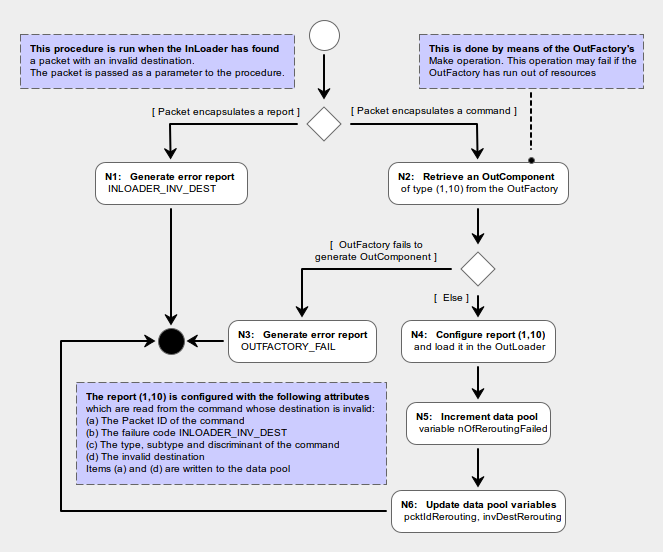
\includegraphics[scale=0.415,keepaspectratio=true]{CrPsPcktReroutingFail.png}
 \caption{Packet Rerouting Failure Procedure}
 \label{fig:PcktReroutingFail}
\end{figure}

\begin{figure}[htbp]
 \centering
 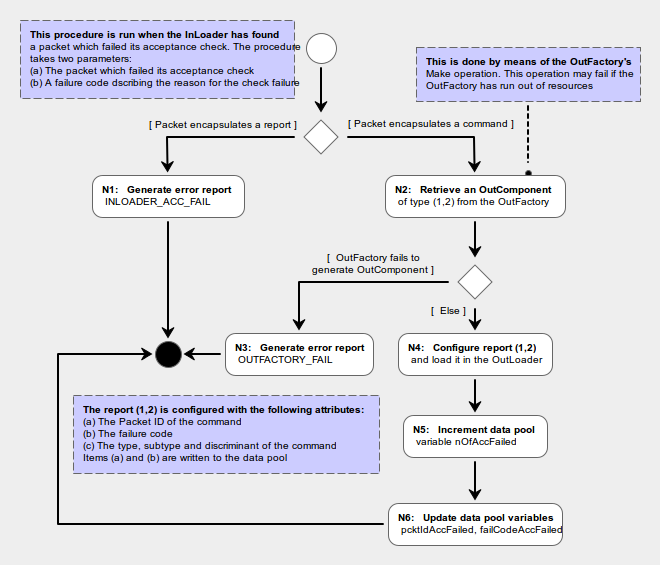
\includegraphics[scale=0.414,keepaspectratio=true]{CrPsPcktAccFail.png}
 \caption{Packet Acceptance Failure Procedure}
 \label{fig:PcktAccFail}
\end{figure}

\begin{figure}[htbp]
 \centering
 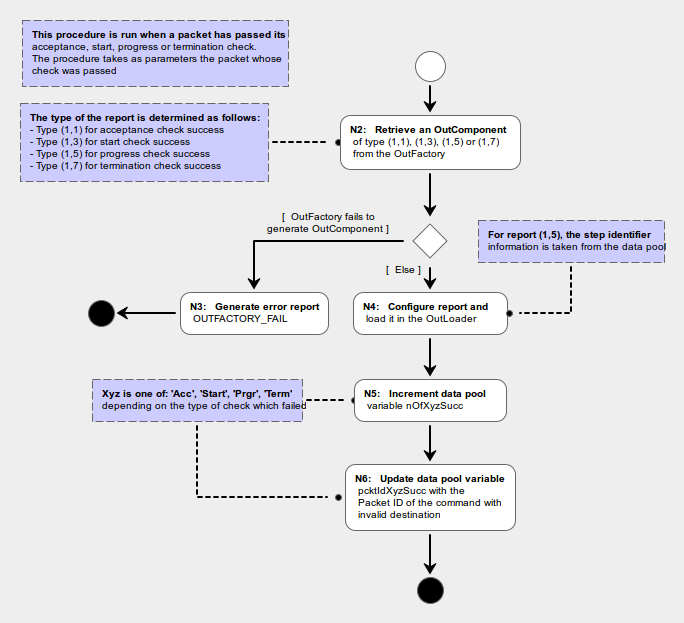
\includegraphics[scale=0.415,keepaspectratio=true]{CrPsCmdVerSucc.png}
 \caption{Command Verification Success Procedure}
 \label{fig:CmdVerSucc}
\end{figure}

\begin{figure}[htbp]
 \centering
 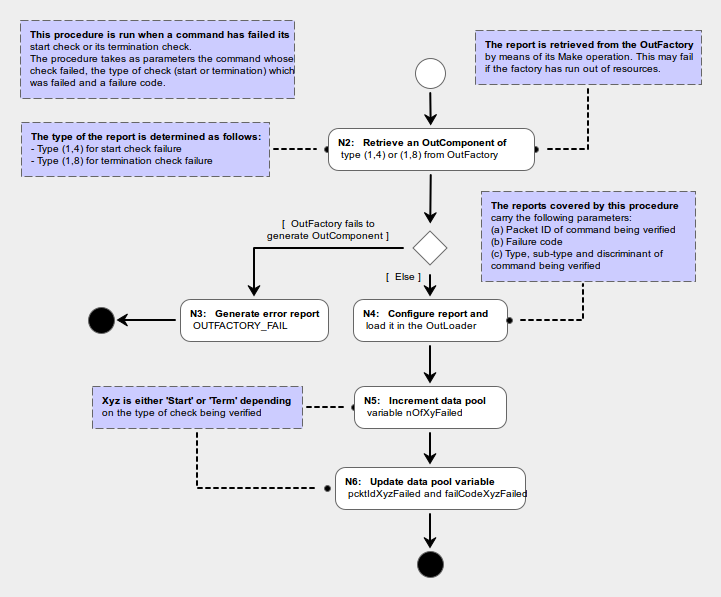
\includegraphics[scale=0.415,keepaspectratio=true]{CrPsCmdVerFail.png}
 \caption{Command Verification Failure Procedure}
 \label{fig:CmdVerFail}
\end{figure}

\begin{figure}[htbp]
 \centering
 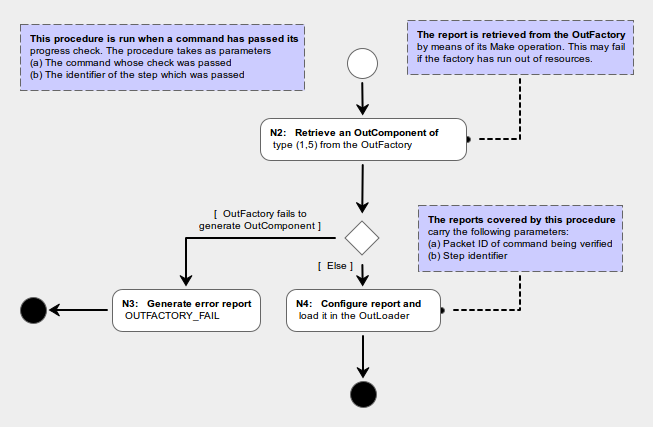
\includegraphics[scale=0.415,keepaspectratio=true]{CrPsCmdPrgrSucc.png}
 \caption{Command Progress Success Procedure}
 \label{fig:CmdPrgrSucc}
\end{figure}

\begin{figure}[H]
 \centering
 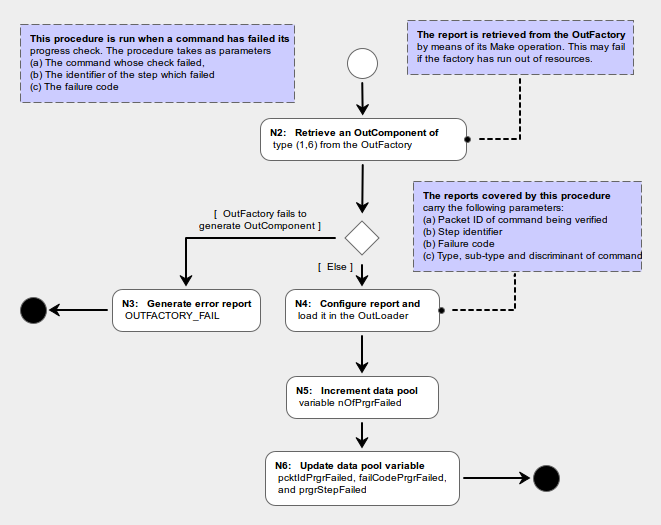
\includegraphics[scale=0.415,keepaspectratio=true]{CrPsCmdPrgrFail.png}
 \caption{Command Progress Failure Procedure}
 \label{fig:CmdPrgrFail}
\end{figure}


%=============================================================================================
\section{Test Service}\label{sec:serv17}
The service type of the Test Service is 17. The PUS Extension of the CORDET Framework supports this service in full.

The Test Service provides the capability to perform two kinds of connections tests: the \textit{Are-You-Alive Test} and the \textit{Is-Application-Process-Alive Test}.

The Are-You-Alive test is like a ping test: an external user sends a command of type (17,1) to the application and the application responds by sending to the user a (17,2) report. Neither the (17,1) command nor the (17,2) report carry any parameters. 

In the Is-Application-Process-Alive Test, an external user sends a command of type (17,3) to application A asking it to perform a connection test with some other application B. Application B is specified through a parameter carried by the (17,3) command. The connection test is not specified by the PUS. The PUS Extension of the CORDET Framework implements it as an Are-You-Alive Test from application A to application B. If this Are-You-Alive Test is successful, application A generates a (17,4) report to its user. The Are-You-Alive Test is declared successful if a (17,2) report from application B is received within time \texttt{AreYouAliveTimeOut} from the sending of the (17,1) command.

%=============================================================================================
\subsection{Service 17 Command and Report Definition}
In the CORDET Framework an out-going report is encapsulated in an OutComponent component and an incoming command is encapsulated in an InCommand component. The framework extension accordingly offers the following components to implement the two commands and the two reports of service 17:

\begin{fw_itemize}
\item Component AreYouAliveCmd implements command (17,1) 
\item Component AreYouAliveRep implements report (17,2) 
\item Component IsAppProcAliveCmd implements command (17,3)  
\item Component IsAppProcAliveRep implements report (17,4) 
\end{fw_itemize}

These components are defined by the way they close the adaptation points of the OutComponent and InCommand. This is defined formally in tables \ref{tab:AP-S17-1} to \ref{tab:AP-S17-4} but the main points are as follows.

The AreYouAliveCmd commmand implements a Progress Action which creates and loads the AreYouAliveRep report. The report destination is the same as the source of the AreYouAliveCmd command. Thus, the processing of the AreYouAliveCmd command consists in sending an AreYouAliveRep to the source of the AreYouAliveCmd. The AreYouAliveCmd commmand is always accepted and it is always started, executed and terminated successfully.

The IsAppProcAliveCmd command is always accepted. The command carries as its single parameter the identifier of the application with which the connection test must be performed. The Start Action of the command verifies the legality of this application identifier. In order to establish its legality, service 17 maintains parameter \texttt{isAppProcAliveDestLst} to hold the list of legal targets for the Is-Application-Process-Alive test. If the application identifier carried by the IsAppProcAliveCmd command is not included in this list, its Start Action is deemed to have failed. The Start Action of the IsAppProcAliveCmd command is shown in figure \ref{fig:Cmd17s3Start} as an activity diagram.

If, instead, the legality of the target application identifier is confirmed, the Start Action sends an AreYouAliveCmd command to the target application. Normally, the target application should respond by sending it an AreYouAliveRep report. If the expected response (the AreYouAliveRep report) is not received within time \texttt{areYouAliveTimeOut}, the command is deemed to have failed its execution.

The mechanism through which the AreYouAliveRep report notifies the IsAppProcAliveCmd command of its arrival is as follows:

\begin{fw_itemize}
\item The service 17 maintains integer \texttt{areYouAliveSrc}
\item The Start Action of the IsAppProcAliveCmd command resets \texttt{areYouAliveSrc} to zero
\item The Update Action of the incoming report AreYouAliveRep loads its source in \texttt{areYouAliveSrc}
\item The Progress Action of the IsAppProcAliveCmd command only declares the command to have successfully terminated if, within time-out \texttt{areYouAliveTimeOut}, it finds \texttt{areYouAliveSrc} equal to the identifier of the application with which the connection test is done
\end{fw_itemize}

One implication of this mechanism is that only one Is-Application-Process-Alive Test may be active at a given time (i.e. the user should only send a new IsAppProcAliveCmd command to an application after execution of the previous IsAppProcAliveCmd command has completed). This constraint is not enforced by the framework and is under the responsibility of the user of the service.

The time-out parameter \texttt{areYouAliveTimeOut} is the same for all target applications. There is, in other words, an underlying assumption that the response time of all target applications is similar and that there is therefore no need to maintain separate time-outs for each target application. If this assumption is not satisfied, the user must update the value of \texttt{areYouAliveTimeOut} with service TBD before starting an Is-Application-Process-Alive Test.



%---------------------------------------------------------------------------------
\subsection{Service 17 Observables}\label{sec:serv17Obs}
Service 17 maintains and makes available in the data pool one single observable listed in table \ref{tab:Obs-S17}.

\begin{cr_obs}{S17}{Observables for Service 17 (Test Service)}
\end{cr_obs}

%---------------------------------------------------------------------------------
\subsection{Service 17 Parameters}\label{sec:serv17Par}
Service 17 maintains and makes available in the data pool the parameters listed in table \ref{tab:Par-S17}.

\begin{cr_par}{S17}{Parameters for Service 17 (Test Service)}
\end{cr_par}

%---------------------------------------------------------------------------------
\subsection{Service 17 Adaptation Points}\label{sec:serv17AP}
The test service consists of two commands and two reports. Commands are defined by the way they close the adaptation points of the InCommand component and reports are defined by the way they close the adaptation points of the OutComponent component. Four tables are accordingly shown below which define the close-out for the adaptation points of the two commands and two reports of service 17.

The following considerations apply to the service 17 commands and reports:

\begin{fw_itemize}
\item The service 17 commands execute in 'one-shot' mode and therefore do not generate progress reports.
\item Service 17 reports are generated unconditionally and hence their enable check always returns 'report enabled'.
\item Service 17 reports are generated as soon as the condition which triggered them occur and hence their ready check always returns 'ready'
\item Service 17 reports are 'one-off' reports and hence their repeat check always returns 'no repeat'
\end{fw_itemize}

\begin{cr_ap}{S17-1}{Adaptation Points for (17,1) Command}
\end{cr_ap}

\begin{cr_ap}{S17-2}{Adaptation Points for (17,2) Report}
\end{cr_ap}

\begin{cr_ap}{S17-3}{Adaptation Points for (17,3) Command}
\end{cr_ap}

\begin{cr_ap}{S17-4}{Adaptation Points for (17,4) Report}
\end{cr_ap}

%---------------------------------------------------------------------------------
\subsection{Service 17 Requirements}
The table in this section lists requirements for the test service.

\begin{cr_req}{S17}{Requirements for Service 17 (Test Service)}
\end{cr_req}

\newpage
\begin{figure}[H]
 \centering
 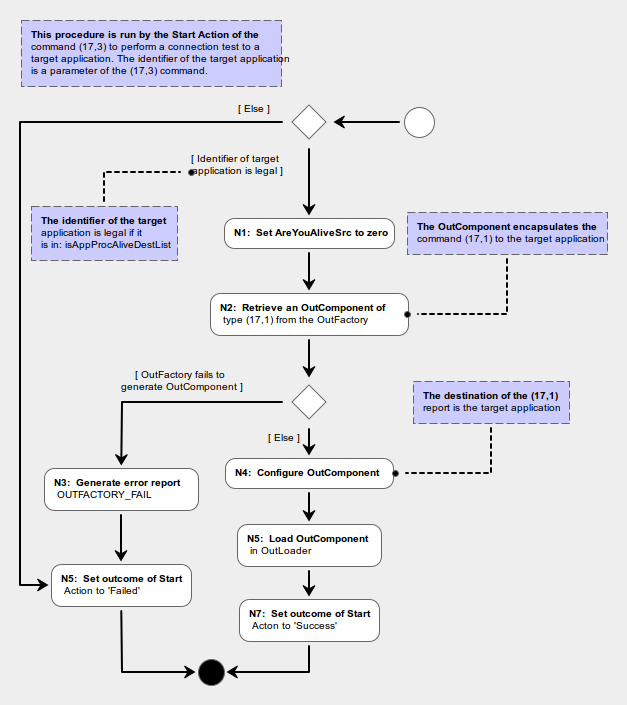
\includegraphics[scale=0.415,keepaspectratio=true]{CrPsCmd17s3Start.png}
 \caption{Start Action of Command IsAppProcAliveCmd Command (17,3)}
 \label{fig:Cmd17s3Start}
\end{figure}

\newpage
\begin{figure}[H]
 \centering
 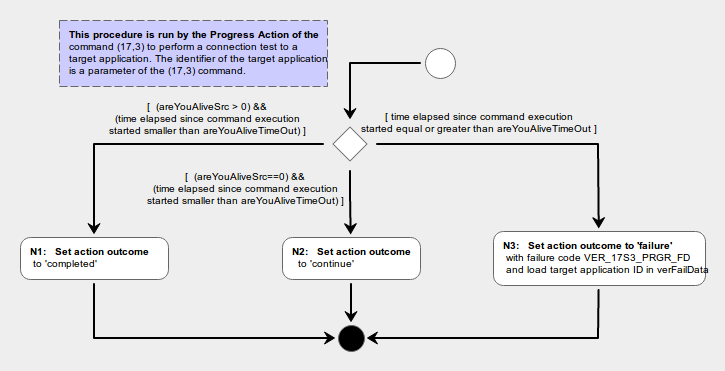
\includegraphics[scale=0.415,keepaspectratio=true]{CrPsCmd17s3Prgr.png}
 \caption{Progress Action of Command IsAppProcAliveCmd Command (17,3)}
 \label{fig:Cmd17s3Prgr}
\end{figure}





\newpage
\appendix
%=============================================================================================
\section{Error Reports}\label{sec:errRep}
The table in this section lists all the error reports which are generated by the PUS Extension of the CORDET Framework. For each error report, the following information is provided:

\begin{fw_itemize}
\item The name of the error report
\item The severity of the error using the same severity level defined for service 5 reports
\item The description of the error report
\item The parameters carried by the error report
\end{fw_itemize}

\begin{landscape} 

\begin{longtable}{|l|c|>{\raggedright\arraybackslash}p{6.0cm}|>{\raggedright\arraybackslash}p{7cm}|c|>{\raggedright\arraybackslash}p{7cm}|}
\caption{Error Reports}\label{tab:errRep}\\
\hline
\rowcolor{light-gray}
\textbf{Name} & \textbf{Sev.} & \textbf{Description} & \textbf{Parameters}\\
\hline\hline
\endfirsthead
\rowcolor{light-gray}
\textbf{Name} & \textbf{Sev.} & \textbf{Description} & \textbf{Parameters}\\
\hline\hline
\endhead
\DTLforeach*{dbErr}{\name=Name,\severity=Severity,\description=Description,\parameters=Parameters}
{\DTLiffirstrow{}{\\\hline}\name & \severity & \description & \parameters}\\\hline
\end{longtable}

\end{landscape}

%=============================================================================================
\section{Request Verification Failure Codes}\label{sec:reqVerFailCodes}
Request verification failure reports of service 1 carry a failure code. The table in this section lists all the failure codes supported by the PUS Extension of the CORDET Framework. The data associated to each failure report depends exclusively on the report sub-type and is specified by the close-out of adaptation point OCM-12 for service reports (see also section \ref{sec:serv1RepDef}.

\begin{longtable}{|l|>{\raggedright\arraybackslash}p{8.0cm}}
\caption{Request Verification Failure Codes}\label{tab:reqVerFailCodes}\\
\hline
\rowcolor{light-gray}
\textbf{Name} & \textbf{Description} \\
\hline\hline
\endfirsthead
\rowcolor{light-gray}
\textbf{Name} & \textbf{Description} \\
\hline\hline
\endhead
\DTLforeach*{dbReqVerFailCodes}{\name=Name,\description=Description}
{\DTLiffirstrow{}{\\\hline}\name & \description}\\\hline
\end{longtable}




%=============================================================================================
\section{PUS Requirements Compliance Matrix}\label{sec:PusReqSOC}
The table in this section presents the level of compliance achieved by the PUS Extension of the CORDET Framework to the PUS requirements of AD-1. The first two columns give the identifier and the text of the PUS requirement. The third column gives the compliance status which can be one of the following:

\begin{fw_itemize}
\item [C1] The requirement is directly implemented by the PUS Extension of the CORDET Framework or by the CORDET Framework itself (i.e. applications instantiated from the framework are guaranteed to be compliant with the requirement)
\item [C2] The requirement may be implemented by applications instantiated from the PUS Extension of the CORDET Framework (i.e. applications instantiated from the framework may be made be compliant with the requirement)
\item [NC] The requirement is not compatible with the PUS Extension of the CORDET Framework (i.e. applications instantiated from the framework cannot be compliant with the requirement)
\item [NA] The requirement is not covered by the PUS Extension of the CORDET Framework
\end{fw_itemize}

In some cases, the compliance level is declared to be 'C1/C2' when part of the requirement is implemented by the PUS Extension of the CORDET Framework and part is left to the application developers.

The fourth column in the table provides the following additional information:

\begin{fw_itemize}
\item [C1] Traceability to the framework requirements implementing the PUS requirement 
\item [C2] Traceability to the adaptation point(s) where application developers can insert their own requirements to achieve compliance
\item [NC] Justification for non-compliance
\item [NI] Indication of whether the requirement might be covered in a future extension of the framework
\end{fw_itemize}


\begin{landscape} 

\begin{longtable}{|c|>{\raggedright\arraybackslash}p{3.0cm}|>{\raggedright\arraybackslash}p{7cm}|c|>{\raggedright\arraybackslash}p{7cm}|}
\caption{Mapping of PUS Requirements to CORDET Requirement}\label{tab:mappingPusToCr}\\
\hline
\rowcolor{light-gray}
\textbf{N} & \textbf{Title} & \textbf{Requirement} & \textbf{C} & \textbf{Justification}  \\
\hline\hline
\endfirsthead
\rowcolor{light-gray}
\textbf{N} & \textbf{Title} & \textbf{Requirement} & \textbf{C} & \textbf{Justification}  \\
\hline\hline
\endhead
\DTLforeach*{dbPus}{\reqN=ReqN,\reqTitle=ReqTitle,\reqText=ReqText,\status=Status,\justification=Justification}
{\DTLiffirstrow{}{\\\hline}\reqN & \reqTitle & \reqText & \status & \justification}\\\hline
\end{longtable}

\end{landscape}




\end{document}  




